\section{H-Bridge}
The H-bridge see \figref{Hbridge} is a commonly used circuit for motor control. To control the motor some FET(s) are controlled with a PWM signal. The duty cycle of this PWM signal determines at which velocity the motor will run.

\begin{figure}[H]
	\centering
	\includegraphics[scale=.6]{figures/Hbridge.pdf}
	\flushleft
	\caption{Standard H-bridge}
	\label{Hbridge}
\end{figure}


There exists a wide range of configurations in which the H-bridge can be implemented. These configurations determines the modes of operation, where each mode has some different properties. Some of the common modes are described in the following sections.

\subsection{Regenerative Coast Mode}

\begin{figure}[H]
	\centering
	\includegraphics[scale=.6]{figures/HbridgeClockwiseCoastON.pdf}
	\flushleft
	\caption{Clockwise coast operation in on-state}
	\label{figures/HbridgeClokwiseCoastON}
\end{figure}

\begin{figure}[H]
	\centering
	\includegraphics[scale=.6]{figures/HbridgeClockwiseCoastRegen.pdf}
	\flushleft
	\caption{Clockwise coast operation in off-state}
	\label{HbridgeClokwiseCoastRegen}
\end{figure}

\subsection{4Q Mode}

\begin{figure}[H]
	\centering
	\includegraphics[scale=.6]{figures/HbridgeClockwise4Q.pdf}
	\flushleft
	\caption{Clockwise 4Q operation}
	\label{HbridgeClokwise4Q}
\end{figure}

\begin{figure}[H]
	\centering
	\includegraphics[scale=.6]{figures/HbridgeCounterClockwise4Q.pdf}
	\flushleft
	\caption{Counterclockwise 4Q operation}
	\label{HbridgeCounterClokwise4Q}
\end{figure}

\subsection{Brake Mode}

\begin{figure}[H]
	\centering
	\includegraphics[scale=.6]{figures/HbridgeClockwiseBrakeON.pdf}
	\flushleft
	\caption{Clockwise brake operation in on-state}
	\label{HbridgeClockwiseBrakeON}
\end{figure}

\begin{figure}[H]
	\centering
	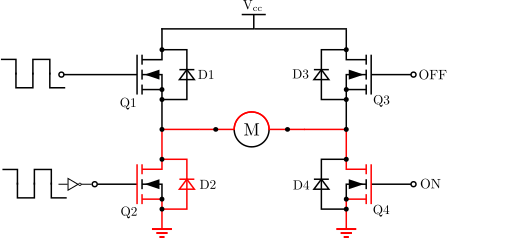
\includegraphics[scale=.6]{figures/HbridgeClockwiseBrakeOFF.pdf}
	\flushleft
	\caption{Clockwise brake operation in off-state}
	\label{HbridgeClockwiseBrakeOFF}
\end{figure}